% Author: Izaak Neutelings (June 2017)
% Updated: December 2022
\documentclass[border=3pt,tikz]{standalone}
\usepackage[outline]{contour} % glow around text
\tikzset{>=latex} % for LaTeX arrow head
\usetikzlibrary{angles,quotes} % for pic (angle labels)
\usetikzlibrary{arrows.meta} % for arrow head size
\usetikzlibrary{bending} % for bending arrow head
\contourlength{1.5pt}

% TIKZ STYLES
\tikzstyle{eta line}=[->,black!60!red,thick,line cap=round]
\tikzstyle{theta node}=[black,pos=0.7,fill=white,scale=0.8,
                       inner sep=1.5pt,rounded corners=3pt]
\tikzstyle{mysmallarrow}=[-{Latex[length=3,width=2.5]},draw=black,line width=0.6,
                          angle radius=45,angle eccentricity=1.1]

\begin{document}

% PSEUDORAPIDITY with manual for-loop over theta, eta
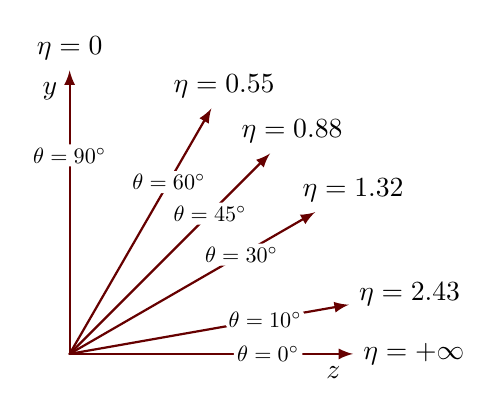
\begin{tikzpicture}[scale=3]
  \message{^^JPseudorapidity simple}
  \def\R{1.2} % radius/length of lines
  \node[scale=1,below left=1] at (0,\R) {$y$}; % y axis
  \node[scale=1,below left=1] at (\R,0) {$z$}; % z axis
  \foreach \t/\e in {90/0,60/0.55,45/0.88,30/1.32,10/2.43,0/+\infty}{ % loop over theta/eta
    \pgfkeys{/pgf/number format/precision=2}
    \draw[eta line] % eta lines
      (0,0) -- (\t:\R) node[anchor=180+\t,black] {$\eta=\e$}
      node[theta node] {$\theta=\t^\circ$};
  }
  %\draw[black!60!red,thick] (0,0.1*\R) |- (0.1*\R,0) ; % overlap in corner
\end{tikzpicture}


% PSEUDORAPIDITY with automatic calculation of eta
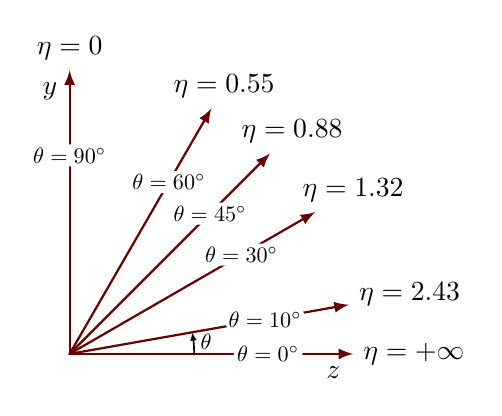
\begin{tikzpicture}[scale=3]
  \message{^^JPseudorapidity with automatic calculation of eta}
  \pgfkeys{/pgf/number format/precision=2} % two decimals
  \def\R{1.2} % radius/length of lines
  \node[scale=1,below left=1] at (0,\R) {$y$}; % y axis
  \node[scale=1,below left=1] at (\R,0) {$z$}; % z axis
  \coordinate (O) at (0,0); % origin
  \foreach \t in {90,60,45,30,10,0}{ % loop over theta
    \ifnum \t = 0
      \def\e{+\infty} % infinity symbol
    \else
      \pgfmathparse{-ln(tan(\t/2))} % pseudorapidity
      %\pgfmathroundto{\pgfmathresult} % round without traling zeroes
      \pgfmathroundtozerofill{\pgfmathresult} % round with trailing zeroes
      \pgfmathsetmacro\e{\t==90?0:\pgfmathresult} % no trailing zeroes for theta = 0
    \fi
    \draw[eta line] % eta lines
      (O) -- (\t:\R) coordinate(P\t) node[anchor=180+\t,black] {$\eta=\e$}
      node[theta node] {$\theta=\t^\circ$};
  }
  %\draw[black!60!red,thick] (0,0.1*\R) |- (0.1*\R,0) ; % overlap in corner
  \draw pic["$\theta$"scale=0.8,mysmallarrow] {angle = P0--O--P10}; % arrow label
\end{tikzpicture}


% PSEUDORAPIDITY including negative side
\begin{tikzpicture}[scale=3]
  \message{^^JPseudorapidity including negative side}
  \pgfkeys{/pgf/number format/precision=2} % two decimals
  \def\R{1.2} % radius/length of lines
  \node[scale=1,below left=1] at (0,\R) {$y$}; % y axis
  \node[scale=1,below left=1] at (\R,0) {$z$}; % z axis
  \foreach \t in {180,170,150,135,120,90,60,45,30,10,0}{ % loop over theta
    \ifnum \t = 0
      \def\e{+\infty} % infinity symbol
    \else \ifnum \t = 180
      \def\e{-\infty} % infinity symbol
    \else
      \pgfmathparse{-ln(tan(\t/2))} % pseudorapidity
      \pgfmathroundtozerofill{\pgfmathresult} % round with trailing zeroes
      \pgfmathsetmacro\e{\t==90?0:\pgfmathresult} % no trailing zeroes for theta = 0
    \fi \fi
    \draw[eta line] % eta lines
      (0,0) -- (\t:\R) coordinate(P\t) node[anchor=180+\t,black] {$\eta=\e$}
      node[theta node] {$\theta=\t^\circ$};
  }
  %\draw[black!60!red,thick] (0,0.1*\R) |- (0.1*\R,0) ; % overlap in corner
  \draw pic["$\theta$"scale=0.8,mysmallarrow] {angle = P0--O--P10}; % arrow label
\end{tikzpicture}


% PSEUDORAPIDITY: plot eta vs. theta
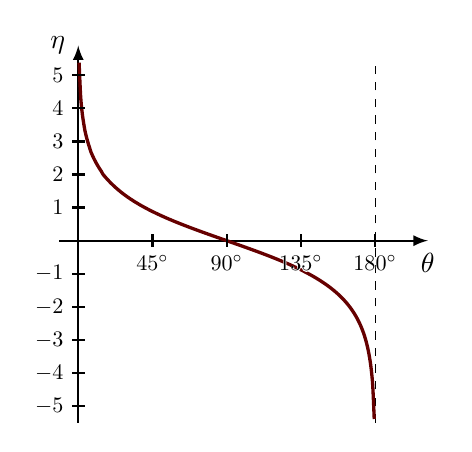
\begin{tikzpicture}[scale=1.2,x=1cm,y=0.35cm,tick/.style={thick,scale=0.8}]

  % SETTINGS
  \def\ltick{2pt} % length of ticks
  \def\xmax{3.7} % maximum x (theta)
  \def\ymax{5.5} % maximum y (eta)
  \pgfmathsetmacro\tmax{2*atan(exp(-0.98*\ymax))} % maximum theta
  \message{^^J ymax = \ymax => tmax = \tmax}
  
  % AXIS
  \draw[->,thick] (0,-\ymax) -- (0,\ymax+0.4) % y axis
    node[left=1] {$\eta$};
  \draw[->,thick] (-0.2,0) -- (\xmax,0) % x axis
    node[below=1] {$\theta$};
  \draw[dashed] (pi,-\ymax) --++ (0,2*\ymax); % asymptote
    
  % PLOT
  \draw[very thick,black!60!red,samples=200,smooth,variable=\t,domain={\tmax:180-\tmax}]
    plot({rad(\t)},{-ln(tan(\t/2))});
  
  % TICKS
  \foreach \t in {45,90,...,180}{ % loop over theta
    \draw[thick] ({rad(\t)},\ltick) --++ (0,-2*\ltick) % x tick
      node[tick,below] {\contour{white}{$\t^\circ$}};
  }
  \foreach \e in {1,...,5}{ % loop over eta
    \draw[thick] (\ltick,\e) --++ (-2*\ltick,0) % y tick
      node[tick,left] {$\e$};
    \draw[thick] (\ltick,-\e) --++ (-2*\ltick,0) % y tick
      node[tick,left] {$-\e$};
  }
  
\end{tikzpicture}

\end{document}